\documentclass[conference]{IEEEtran}
%http://wp.internetsociety.org/ndss/wp-content/uploads/sites/25/2017/09/bare_NDSS.tex
\usepackage[utf8]{inputenc}
\usepackage[colorlinks = true,
            linkcolor = blue,
            urlcolor  = blue,
            citecolor = green,
            anchorcolor = blue]{hyperref}

\usepackage{graphicx}
\graphicspath{{figs/}}
\usepackage{booktabs}

\begin{document}
\title{Non-secure dynamic updates in DNS}

\author{\IEEEauthorblockN{Author1}
\IEEEauthorblockA{Institution1\\
someemail@somedomain.com}
\and
\IEEEauthorblockN{Author2}
\IEEEauthorblockA{Institution2\\
someemail@somedomain.com}
\and
\IEEEauthorblockN{Author3}
\IEEEauthorblockA{Institution3\\
someemail@somedomain.com}}

\maketitle



\begin{abstract}
The abstract goes here.
\end{abstract}

\section{Introduction}


\section{Background}


In this section, we introduce the necessary background about the dynamic updates in DNS, its security considerations and common software implementations.

\begin{comment}
\subsection{Brief History}
\michal{Not sure if going so far back is necessary}
The basic specification of the domain name system was introduced over 30 years ago \cite{rfc1035,rfc1034}. 
Before then, host name to address mappings were maintained by the Network Information Center (NIC) in a single file called \texttt{HOSTS.TXT} and distributed by all hosts using FTP \cite{rfc952,rfc953}.
%
The DNS protocol initially supported queries of a statically configured database that was updated manually as it was not expected to change rapidly \cite{rfc1034}. 
However, with the introduction of the Dynamic Host Configuration Protocol (DHCP) \cite{rfc2131}, which allows to dynamically assign an IP address to each device on a network, the automatic reconfiguration mechanism for DNS  became essential.
\end{comment}

\subsection{Dynamic Updates in DNS}
%The DHCP protocol provides not only a mechanism for allocation of network addresses to Internet hosts but also can be configured to  dynamically update both the \texttt{A} and \texttt{PTR} (reverse DNS record) resource records in the DNS server on a client's behalf.
%%MK: \michal{Should be shortened and more to the point I guess}
%%MK: Internet services may use static IP addresses but can also dynamically change over short periods of time, on the order of hours or days \cite{gio}.
%%MK: Due to the distributed nature of the domain mane system and the proliferation of its actors such as registrars or registry operators, updates to the global domain name system may take hours to propagate. 
%
\textit{Dynamic updates in DNS} is a protocol extension that addresses the problem of fast changes of DNS resource records (RRs) in zone files, such as an \texttt{A} record, which provides a mapping between a domain name and an IP address.

The dynamic updates have been described in RFC 2136 \cite{rfc2136} in 1997. 
%%MK: The specification supports all DNS record types.
%%MK: Therefore, 
A client can update, add or delete almost any type of record, including \texttt{A}, \texttt{AAAA}, \texttt{NS}, or \texttt{TXT}.
It is often used %as an extension of
in combination with the DHCP protocol, which can be configured %not only 
as a mechanism for allocation of network addresses to Internet hosts but also to dynamically update both \texttt{A} and \texttt{PTR} (pointer or reverse DNS) resource records in the DNS server %on a client's behalf 
on behalf of its clients (cf.~\autoref{fig_dhcp}).

\begin{figure}[!ht]
\centering
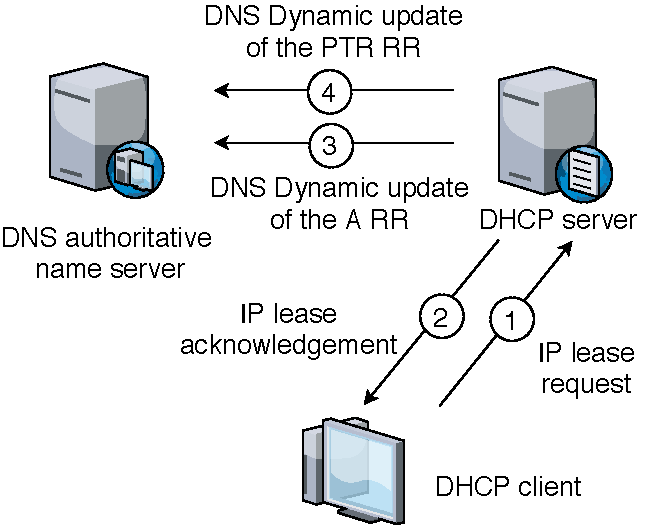
\includegraphics[width=2.5in]{figs/dhcp.pdf}
\caption{The DHCP server can be configured to register and dynamically update the host (\texttt{A}) and pointer (\texttt{PTR}) resource records with the authoritative DNS server of the zone on behalf of its DHCP-enabled clients.
%https://docs.microsoft.com/en-us/previous-versions/windows/it-pro/windows-server-2008-R2-and-2008/dd145315(v=ws.10)
}
\label{fig_dhcp}
\end{figure}

%It supports all DNS record types, but often it is used only as an extension of the DHCP system, and in which the authorized DHCP servers register the client records in the DNS.


%
%Following this specification, a DNS client can add or delete any type of RR, such as A, AAAA, CNAME, or NS.

%Some servers that are maintained by certain types of Internet service providers (ISPs) are likely to change their IP address over very short periods of time, 


\begin{comment}
The proposed DNS \texttt{UPDATE} message complies with the standard DNS message format (cf. RFC 1035 \cite{rfc1035}) and is defined as follows:
\newline
\noindent
       \texttt{+----------------+}
      \newline \noindent
       \texttt{|\hspace{0.85cm} Header\hspace{0.85cm} |} contains the opcode value~(5)
      \noindent \texttt{+----------------+}
      \newline \noindent
      \texttt{|\hspace{1.16cm}Zone\hspace{1.16cm} |} specifies the zone to update
      \texttt{+----------------+}
      \newline \noindent
      \texttt{|~\hspace{0.115cm}~Prerequisite\hspace{0.115cm} |} RRs that must~(not)~preexist
      \texttt{+----------------+}
      \newline \noindent
      \texttt{|\hspace{0.95cm}Update\hspace{0.95cm} |} RRs to be added or deleted
      \texttt{+----------------+}
      \newline \noindent
      \texttt{|\hspace{0.005cm}Additional Data\hspace{-0.005cm} |} additional information (if any)
      \texttt{+----------------+}
\end{comment}


The \texttt{UPDATE} message complies with the standard DNS %message
format (cf. RFC 1035 \cite{rfc1035}).
The \texttt{Header} section contains the \texttt{UPDATE} opcode equal to~5. The \texttt{Zone} section must specify the zone name to update, i.e. a domain name (e.g.: \texttt{\url{example.com}}). The \texttt{Prerequisite} section can specify 
requirements %demanded as conditions for an update in terms of a DNS zone file content 
that must be satisfied by the DNS zone file such as existence or nonexistence of a specific resource record. % (RR). %, before being allowed to proceed with an update
The \texttt{Update} section contains resource record(s) to be added to or deleted from the DNS zone (e.g.:  \texttt{\url{example.com} A 10.10.10.10}), whereas \texttt{Additional Data} section can be used to supply a server with some additional information needed to, for example,  secure DNS update~\cite{rfc2136}.

When a primary master name server that supports dynamic updates receives an update request, it verifies whether all prerequisites (if any) defined by the %requestor 
client are met and whether restrictions (if any) regarding which hosts are permitted to make updates are met.
Note that if there are no restrictions defined by the authoritative name server, anyone who knows the name of the zone (e.g.: \texttt{\url{example.com}}) and the name server (e.g.: \texttt{\url{ns1.example.com}}) for that zone is capable of updating its content by sending a single UDP datagram.
%MK: It can be tested using a standard \texttt{nsupdate} command\footnote{Dynamic DNS update utility: \url{https://linux.die.net/man/8/nsupdate}}.
%
%
The RFC specification also defines a case, where the request is sent to a DNS slave server that is authoritative for a given domain name.
The update request is expected to be forwarded towards the primary DNS server that can modify the zone file.

\subsection{Security Considerations}
The method described in RFC 2136 %also includes a brief discussion of 
briefly discusses the security considerations and recommends using DNS Security Extensions (DNSSEC) digital signatures covering requests to secure dynamic updates and restrict %requestors 
clients to those authorized to perform them %, for example, a local DHCP server 
(cf. RFC~2137~\cite{rfc2137} %, superseded by RFC~3007~\cite{rfc3007}).
and RFC~3007~\cite{rfc3007}).
If the public key security mechanism is not implemented, an authoritative name server is expected to accept the dynamic updates only from a statically preconfigured set of IP addresses.
The address match lists should be as restrictive as possible and limited to, for example, an IP address of a DHCP server.
An alternative security mechanism based on shared secret key (TSIG: Secret Key Transaction Authentication for DNS) and message authentication code was introduced three years later in RFC 2845 \cite{rfc2845} and became the most commonly used method in popular DNS software implementations.
%
%
The pressing need for DNS dynamic updates and the delayed introduction of the robust and lightweight security measures may explain a rapid uptake of the vulnerable by design, non-secure dynamic updates.
%why the vulnerable, non-secure implementations have

%and the protocol's simplicity caused a rapid uptake of the specification.


\subsection{Implementations of Dynamic Updates}

The common implementations of the DNS software, such as the open source Linux BIND \cite{bind} or the Microsoft Server DNS support vulnerable configurations, such as accepting requests from all hosts.
Some are vulnerable by default.

Microsoft Server supports two configurations of a DNS server: an active directory--integrated or a standard primary zone.
To date, both versions support vulnerable to %MK: zone poisoning 
non-secure dynamic updates configurations.
The former allows either ``secure only" updates using extended TSIG or ``nonsecure and secure'' updates. %MK: , whereas the latter 
Standard primary zone configuration supports \textit{only} ``nonsecure and secure''  updates.
Microsoft is aware of the vulnerability and informs the users willing to setup a non-secure implementation that ``allowing nonsecure dynamic updates is a significant security vulnerability because updates can be accepted from untrusted sources.''
However, it remains unclear why the vulnerable version is still supported in the latest production version of the software--over 20 years after the initial release of the RFC specification.

Open source DNS software such as BIND or PowerDNS also support non-secure dynamic updates. 
Dynamic update is enabled by including the \texttt{allow-update}  % or an \texttt{update-policy} 
clause in the zone statement in BIND and \texttt{allow-dnsupdate-from} in PowerDNS.
An administrator may configure IP ranges that are allowed to perform DNS updates, in particular ``\texttt{0.0.0.0/0}'', or may use a built-in argument ``\texttt{any}'' in BIND to accept updates from all IP ranges.
%, which means that all ranges are accepted to make DNS updates. 
Both implementations support DNS update forwarding.  
If a slave server receives a DNS dynamic update for a zone for which it is authoritative and the update forwarding is enabled then the request will be forwarded to and processed by the master server.


\begin{comment}
open source DNS software, 

If a slave for a zone receives a DDNS update for a zone for which it is authoritative, it will not update its zone data directly. It will either discard it, or it will forward it to the master. To make the slave forward the DDNS update, you need to configure allow-update-forwarding (see the Administrator Reference Manual for more detail) - this is not enabled by default.
\end{comment}


\subsection{Dynamic Updates and DNSSEC}
DNSSEC is a set of extensions to DNS which provide %to DNS resolvers
authentication of origin and DNS data integrity \cite{rfc4033}.
It provides a solution to malicious path changes between DNS resolvers and authoritative name servers if end-to-end validation is permitted on hosts. 
The current implementations of the DNS software provide a good support for integrating DNSSEC with dynamically updated zones.
It is critical because if the dynamically changed records and the zone are not re-signed automatically, then any user who uses a validating DNS resolver would not be able to make a successful resolution.
BIND 9.7.0 (and later versions) support the semi-automatic smart signing feature and fully automatic zone signing functionality which improve and simplify the process of signing, operating, and maintaining DNSSEC-signed zones (in particular zones updated dynamically).
The \texttt{auto-dnssec maintain} clause in the zone informs the name server that this is a dynamic zone, and therefore it should be automatically signed, and periodically re-signed as necessary.
However, dynamic updates function in BIND integrated with DNSSEC require to authenticate hosts\footnote{using polices defined in the \texttt{update-policy} clause which is mutually exclusive with the \texttt{allow-update} clause which supports non-secure update requests.} and may only be used with a secret key %(TSIG or SIG(0)) 
which is used to cryptographically sign each update.
Similarly, DNSSEC in %Windows Server 2012 
Windows 2008 R2 (and later versions) can also be used for dynamic zones (and automatic re-signing updated zones), but only if part of active-directory integrated zones configured with secure updates.
Therefore, even if DNSSEC does not prevent the zone poisoning attack, the common DNSSEC implementations enforce using secure dynamic updates.


\section{Adversary Model}
%%In this section, we explore the attacks that can be carried out by the adversary. We explain our infrastructure which we used to carry out attack on our victim. Finally, we present the taxonomy of attacks with discussion on their viability, stealthiness and  implications for the domain owners.

In this section, we present the taxonomy of attacks by our adversary using DNS dynamic updates on vulnerable slave server. We briefly explain our setup, followed by the methodology which we used to compromise domain validation. Finally, we discuss the viability and stealthiness of these attacks and also explain the implications for the domain owners. 

%using zone poisoning vulnerability. We discuss the viability and stealthiness of these attacks and also explain the implications for the domain owners.

\subsection{Infrastructure Setup}

In order to explain the adversary model, we set up our infrastructure comprising of two servers. A DNS slave server that is vulnerable to receive  dynamic zone updates (victim) without authentication from any authoritative server. The second server will act as an adversary to update the zone files of our victim.  We explain these configurations in detail below. 


\textbf{Adversary Configuration:} Depending on the type of attack, different configurations might be required. In our setup, we assume our adversary \hl{has access to the compromised machine} \michal{It's a bit confusing to me. Does it mean, that the adversary has like ssh access? Or just that there's connectivity between both hosts? Also the Victim is not yet compromised during the setup, right?} with a public IP address. The adversary will also require Dynamic DNS update utility \texttt{nsupdate} to modify the zone of our victim. Furthermore, for more sophisticated attacks other services like email server and webserver are required. %An email server with forwarding is also required for more sophisticated attacks explained later. EDIT

\textbf{Victim Configuration:} Our victim server is running apache bind software. For the adversary to modify the records victim servers should also be vulnerable with the non-secure update of records explained in the previous section. We assume our victim is hosting a website \texttt{example.com}, which is protected by SSL certificate. The victim server might also have a mail server configured with the mx record configured in the zone file.  


\subsection{Taxonomy of Attacks}
We define the attacks by the adversary in the following three categories. 
%We present the details of the following three types of attacks by the adversary and discuss the viability and stealthiness of these attacks. We also analyze the implications of these attacks on our victim

\begin{itemize}
\item \textbf{Denial of Service (DoS) attack:} In the DoS attack the adversary will be able to disrupt the service of the victim temporarily. It is much easier to execute with limited stealthiness, as the victim would notice the unresponsive domain and would be able to fix the configuration quickly. 


\item \textbf{Man-in-the-Middle (MITM) attack:} MITM attack requires more sophistication from the adversary while being more stealthy and difficult to detect. In this type of the attack, our adversary will comprise the victim zone file and redirect traffic to its server and then back to the victim without getting detected. It can be used to capture the traffic between victim server and its customers.  

\item \textbf{Domain shadowing attack:} Finally, the adversary might be able to spawn malicious domains which he can then use for exploit kits, phishing and stealing information from the victim. Domain shadowing attacks are more stealthy in nature as the subdomains inherit the trust of the parent domain which enables them to evade countermeasures based on domain reputation or blacklisting systems. The attacker can spawn multiple subdomains at no cost can rotate between them to evade detection. Furthermore in Section~\ref{} we explain how attackers can by-pass domain control validation in order to setup SSL certificates. 
\end{itemize}



\subsubsection{Denial of Service (DoS) Attack} 
The DoS attack will only cause limited disruption in the service until the victim gets notified. However, these types of attacks can result in financial losses due to domain downtime or loss of customers. The adversary can cause a DoS attack using one of the following methodologies. 

\textbf{Deletion of A record of domain/sub-domain:} The adversary can delete A record with \texttt{nusupdate} utility command \texttt{update delete example.com A} using nsupdate. This would delete the domain and corresponding IP address of example.com from zone file, resulting in downtime of the traffic. 

\textbf{Deletion of MX records:} Similarly, adversary can also delete MX record which will not only disrupt email service but also hinder any abuse messages sent to victim.  

% Deletion of NS records not possible 
%\textbf{Deletion of NS record:} Deletion of NS record will be most disruptive for the victim as all available domains including email service will be un-accessible to victim and its users till the zone file is updated with correct records. 
 % Need to check following statements...
% Check edit of SOA records .... 


 \textbf{Deletion of delegation:} Delegated zones can be used for variety of purposes. It can be used for management of domains and subdomains or for the backup if master zone is down,  when configured as slave. If adversary successfully deletes delegation in the zone file. It would not only cause service disruption to the  domains handled by delegated server, but would also disrupt backup. 


\subsubsection{Man-in-the-middle (MITM) Attacks}
The second type of attack that adversary can utilize is MITM attack. These attacks can be more sophisticated and harder to detect. 

\textbf{Update of A records:}
Adversary can update the A records in the zone file of the victim and change IP address to its compromised machine. In this way the traffic directed towards the victim will be redirected towards the adversary. If the adversary acts as a proxy server it can gain useful information about the customers of the victims. For instance, the number of customers, geo-location based on IP addresses and pages that were visited by the customers. However, for a more sophisticated attack the adversary can setup a phishing website to steal all the personal information of customers of our victim. He can then forward the collected information back to the customer for an increase stealthiness. 

\textbf{Update of MX records:} 
If the victim runs a mail server, adversary can also change the MX record with its own IP. The adversary in this case can store the emails of the victims and forward the emails back to the victim. If the adversary wants to run a phishing website it can also update the MX record and bypass email challenge to validate the domain. 

%and map its own IP address for the domain. In this case the traffic for his server will be redirected towards to the adversaries server. However, the victim or its customers would be able to detect the outage. If the adversary run a phishing website similar to the victim, he might be able to successfully steal customer information. Similarly, adversary will also be able to build a completely new sub-domain of our victim legitimate domain. He can then use the sub-domain to collect 




%\begin{itemize}
%\item redirect traffic for disruption
%\item add a subdomain and redirect info after stealing 
%\item add a subdomain to launch a phising attack 
%\item add a domain with domain verfication using certs to show as legitimate site 
%\end{itemize}
%\textbf{Add/Update MX record:} 
%\begin{itemize}
%\item redirect all mail to own servers to steal important information 
%\item add another mx record with subdomain to use in phishing scam 
%\item add an mx record with email server configured to by pass domain verification required for SSL certificates
%\end{itemize}


\subsection{Domain Shadowing Attack}

Finally, the adversary can spawn the subdomains for phishing and exploit kit attacks by adding A and AAAA records to the zone files. Furthermore, the attacker can add MX record which can be useful in redirecting abuse emails to the attacker and increase the stealthiness of the attack. 

\textbf{Add A record:} 
Adversary can add an A records for subdoamins with IP address pointing to the server under its control in the victims zone file. He can spawn unlimited number of subdomains and rotate between them to evade detection. Adversary can use the business model of the parent domain and can setup subdomains for phishing attack. The victim would not be able to detect attack unless it is notified. Furthermore, the attacker can use the reputation of the victim's domain to by-pass blacklisting services for the exploit kit attack. It can also lead to adversely impact the reputation of the victim's domain and business after the attack is discovered by various blacklisting services.

\textbf{Add Domain Delegation:}
In order to spawn multiple subdomains and rotations between them the adversary needs to constantly update the zone file of victim. It might alert the victim because to constant changes in the file. In order to improve the stealthiness of this attack adversary can add delegated domain. It can then spawn multiple subdomains on his server without any updates to victim zone file. For example if the adversary add a delegated domain \textttt{accounts.example.com} with the command %check this 
\texttt{nsupdate NS 10.10.10.10 accounts.example.com}. He can then spawn cs.accounts.example.com or any other sibling domains in the zone file of 10.10.10.10 server without any interaction with the victim server. 




\subsection{Compromising Domain Control Validation}


\textbf{ Add MX record:} 
Adversary can also add mx record to victims zone file. It can be useful for particular places, a ) compromise email based challenge for domain control validation. Adversary can also edit SOA records to get the abuse emails further avoid detection.


In our experimental setup we were able to by-pass domain control validation for two different certificate authorities (Let's encrypt and ..). It allowed us to add HTTPS for the domains spawned by our methodology. 



%\section{Threat Model}
\section{Methodology}
\subsection{Datasets descriptions}
\subsection{Ethical considerations}
\subsection{Active scans}

\section{Enumeration of vulnerable resources}

\begin{table}
  \caption{Summary of vulnerable resources \label{tab:vulnerable}}
 \centering
\begin{tabular}{l*{3}{c}}
\Xhline{2\arrayrulewidth}
\#  & \textbf{\textit{Global 1}} & \textbf{\textit{Global 2}} \\
\hline
Domains & 309,687(0.095\%) & 381,965(0.108\%) \\
NS (IP addresses) & 5738(0.166\%) & 5576(0.145\%) \\
Domain--NS IP pairs & 579,186(0.018\%) & 679,930(0.014\%) \\
\Xhline{2\arrayrulewidth}
 \end{tabular}
\end{table}


\subsection{Global campaign 1}
We performed our first global campaign between \hl{need the timeframe here} using domain set specified in Table \ref{tab:data}. We were able to confirm 309,687 vulnerable domains translating into 0.095\% of all the scanned domains and 5738 (0.166\%) unique, vulnerable NSs. In total, we discovered  579,186 (0.018\%) vulnerable Domain--NS pairs (Table \ref{tab:vulnerable}). The low percentage of vulnerable resource can be explained by the broad input set that were not actively verified before vulnerability scans (\ref{sec:dataset}). 

\subsection{Global campaign 2}
Our second global campaign (\hl{need the timeframe here}) confirmed the results obtained during the first trail. We discovered 381,965(0.108\%) vulnerable domains, 5576(0.145\%) vulnerable NSs and 679,930(0.014\%) unique Domain--NS pairs. In comparison to the first global campaign, the number of vulnerable domains was increased by more than 23\%, while the number of vulnerable servers decrease by 3\% regardles the increased input set size. 
\michal{Do we need to explain those results further?}


\subsection{Short-lived domains}


\subsection{Vulnerable subdomains}

\begin{table}
  \caption{Summary of vulnerable subdomains \label{tab:subdomains}}
 \centering
\begin{tabular}{l*{2}{c}}
\Xhline{2\arrayrulewidth}
\#  & \textbf{\textit{Subdomains}}  \\
\hline
Subdomains & 399 / 35382217 (0.001127685\%) \\
NS (IP addresses) & 401 / 722989 (0.055464191\%)  \\
Subdomain--NS IP pairs & 520 / 104955041 (0.00049545\%)  \\
\hline
2nd level domains & 236 \\
Subdomains with vulnerable 2nd level domain &  14 (5.93220339\%) \\
\Xhline{2\arrayrulewidth}
 \end{tabular}
\end{table}

\michal{We should explain here why we have ``low quality'' input set of subdomains}
Table \ref{tab:subdomains} presents the number of detected vulnerable subdomains. We observe 3 orders of magnitude lower number of vulnerable domains than when performing 2nd level domain scans (Figure \ref{tab:vulnerable}), but a comparable number of vulnerable server. This is caused by higher domain dynamism and fast-dissapearing, disposable domains present in the input subdomain list~\cite{chen2014dns}. Furthermore, the input set did not include servers responsible for the majority of vulnerable 2nd level domains (Figure \ref{fig:ip_pie}) explaining the disproportion between the percentage of vulnerable servers and domains. 

Furthermore, we extract 2nd level domains from vulnerable subdomains. Vulnerable subdomains are widely spread between second level domains resulting in ~1.69 subdomains per a 2nd level domain on average. Surprisingly, only 14 (6\%) extracted 2nd level domains were detected as vulnerable during our previous tests. While our study focuses on 2nd level domains, this suggests that multiple subdomain servers are vulnerable to our attack even when the delegating 2nd leve domain servers are properly configured. Finally, we present only servers that responded with a modified entry within a short period of times representing the lowe bound of the problem. 


\subsection{Propagation between primary and secondary name servers}

\begin{table}
  \caption{Domains vulnerability \label{tab:propagation_vulnerable}}
 \centering
\begin{tabular}{l*{3}{c}}
\Xhline{2\arrayrulewidth}
\textbf{\textit{Authoritative}}  & \textbf{\textit{Slave}} & \textbf{\textit{Both}} \\
\hline
12083 & 12487 & 17396 \\
\Xhline{2\arrayrulewidth}
 \end{tabular}
\end{table}



To investigate the vulnerability of different types of servers, we repeat our tests targeting different groups of DNS servers. For each vulnerable domain we prepared a list of primary and secondary name servers based on actively queried \texttt{NS} and \texttt{SOA} records. In the first experiment, we sent injects only to primary servers and queried primary and secondary servers right away and after 24 hours. In our second experiment, we targeted the secondary servers uniquely and again queried all the servers right away and after 24 hours. 

The majority of the domains can be attacked using both their primary and secondary servers (Table \ref{tab:propagation_vulnerable}). However, more than 24,000 domains were vulnerable when attacked using one type of servers. Surprisingly, we discovered a similar amount of domains having vulnerable primary and secondary servers. 

\begin{table}[!htbp]
\centering
\caption{Propagation}
\label{tab:propagation}
\begin{tabular}{@{}lcccc@{}}
\toprule
 & \multicolumn{2}{c}{\textbf{\begin{tabular}[c]{@{}c@{}}Master\end{tabular}}} & \multicolumn{2}{c}{\textbf{\begin{tabular}[c]{@{}c@{}}Slave\end{tabular}}} \\ %\midrule
 & \multicolumn{1}{c}{\textbf{\begin{tabular}[c]{@{}c@{}}0h\end{tabular}}} & \multicolumn{1}{c}{\textbf{\begin{tabular}[c]{@{}c@{}}24h\end{tabular}}}& \multicolumn{1}{c}{\textbf{\begin{tabular}[c]{@{}c@{}}0h\end{tabular}}} & \multicolumn{1}{c}{\textbf{\begin{tabular}[c]{@{}c@{}}24h\end{tabular}}} \\ \midrule
Domains
 & 29479 & 28242 & 29883 & 25268\\ \midrule
Servers
 & 4514 & 4498 & 6526 & 6444\\ \midrule
 Propagation
 & 1643 & 1645 & 15 & 16\\ \bottomrule
\end{tabular}
\end{table}

\begin{figure}[!hbt]
\centering
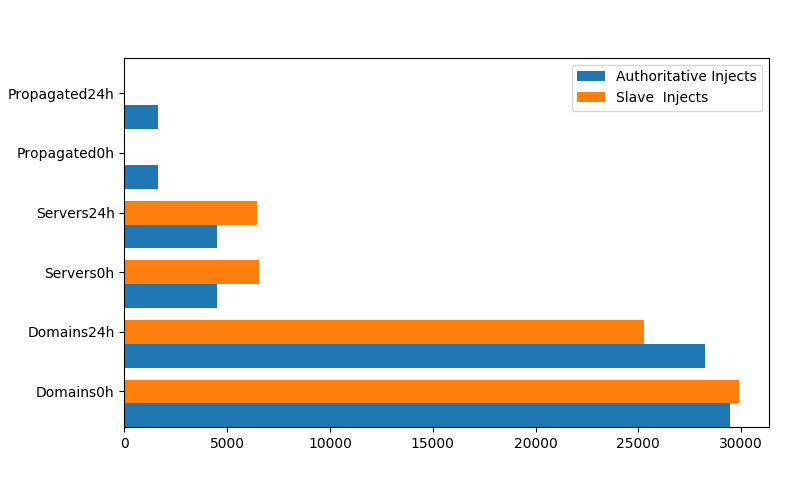
\includegraphics[width=0.8\columnwidth]{propagation}
\caption{Propagation results.}
\label{fig:propagation}
\end{figure}


We then investigate the evolution of the number of affected domains and servers over time (Table \ref{tab:propagation}).\michal{We can use Tab. \ref{tab:propagation} or Fig. \ref{fig:propagation} here} Querying affected domains directly after sending the inject reveals a similar number of domains for both primary and secondary servers. However, after 24h, the entries injected using secondary servers disappear at a much higher rate than those injected using primary servers. The entries disappear when corresponding, unaffected primary server, propagates the correct configuration to the infected secondary server. 

Furthermore, we evaluate the number of servers affected using both types of injects. Targeting primary servers results in a significantly lower number of affected servers. This is because of a higher number of secondary servers for each affected domains. The number of affected servers remains stable throughout our experiment. 

Finally, we investigate if a vulnerable server is able to infect other servers with an updated configuration. When targeting primary servers, we discovered more than 1,600 secondary servers that downloaded the incorrect zone information. We discovered a significantly lower number of secondary servers pushing changes to the primary one. This is understandable, as if configured correctly, secondary servers are not allowed to update zones. In both cases, the number of affected servers increase slightly over time. 

\subsection{Fingerprinting of vulnerable name servers}


\subsection{Fingerprinting of vulnerable name servers}
\section{Descriptive statistics of vulnerable resources}
\subsection{Country overview}
\subsection{Per-AS statistics}
\subsection{Per-CERT statistics}
\subsection{Per-TLD statistics}
\subsection{Popularity of affected domains}

\section{Notifications}

While non-secure dynamic updates have been a well-known misconfiguration issue for years, DNS operators still lack of the proper incentives to act.
To incentive the action of the operators of these vulnerable resources, we conducted a series of notification experiments.

Previous studies have demonstrated that directly notifying  operators does not lead to significant remediation rates~\cite{cetin2017make}. Instead, to increase the remediation rates, we notified the national CERTs and CSIRTs responsible for the hygiene of the networks where the vulnerable DNS servers are located.
Given the high concentration of vulnerable resources in a single country, before sending out the notifications at scale, we contacted directly the Japanese CERT with whom we shared all the information related to these vulnerable resources. After contacting this CERT, we measure a considerable drop (92\%) of vulnerable domains in this country by fixing 29 of the vulnerable servers.


However, even after Japan remediated most of the domains at risk in that country, more than 5,100 servers were still vulnerable leaving more than 43,000 domains at risk being exploited.
In total we conducted 8 email notification campaigns divided into 2 different phases: \textit{Phase1} targeting CERTs and CSIRTs members of the so-called 'Trusted Introducer' community; and  \textit{Phase2} targeting national and governmental CERTs. Table~\ref{tab:notif_campaign} shows an overview of the notifications that were sent out during each phase. In total, more than 200 CERTs and CSIRTs were notified via email during the time span of 6 months. The interaction with these actors was relatively low and less than 10\% actually required additional information about the scanning process. Similarly, less than 5\% of them open an automated ticket and only in 4 occasions we were notified back when the ticket was closed.

\begin{table}[!htbp]
\centering
\caption{Summary of the notification campaigns}
\label{tab:notif_campaign}
\begin{tabular}{@{}llrrr@{}}
\toprule
 & \multicolumn{1}{c}{\textbf{\begin{tabular}[c]{@{}c@{}}Notification\\ Date\end{tabular}}} & \multicolumn{1}{c}{\textbf{\begin{tabular}[c]{@{}c@{}}\#Notified\\ Entities\end{tabular}}} & \multicolumn{1}{c}{\textbf{\begin{tabular}[c]{@{}c@{}}\#Unreachable\\ Entities\end{tabular}}} & \multicolumn{1}{c}{\textbf{\#Replies}} \\ \midrule
Pilot
 & 2017-05-01 & 1 & - & \begin{tabular}[c]{@{}r@{}} 1 manual \end{tabular}\\ \midrule
\multirow{3}{*}{Phase 1} & 2017-09-06 & 44 & 2 & \begin{tabular}[c]{@{}r@{}}7 automatic\\ 16 manual\end{tabular} \\
\multicolumn{1}{c}{} & 2017-09-28 & 35 & 2 & \begin{tabular}[c]{@{}r@{}}6 automatic\\ 13 manual\end{tabular} \\
\multicolumn{1}{c}{} & 2017-10-19 & 27 & 2 & \begin{tabular}[c]{@{}r@{}}4 automatic\\ 7 manual\end{tabular} \\ \midrule
\multirow{4}{*}{Phase 2} 
 & 2018-02-14 & 168 & 5 & \begin{tabular}[c]{@{}r@{}}14 automatic \\ 40 manual \end{tabular}\\
 & 2018-02-28 & 167 & 5 &  \begin{tabular}[c]{@{}r@{}}12 automatic \\ 24 manual \end{tabular} \\
 & 2018-03-16 & 162 & 5 & \begin{tabular}[c]{@{}r@{}}12 automatic \\ 24 manual \end{tabular}  \\
 & 2018-04-12 & 76 & 5 &  \begin{tabular}[c]{@{}r@{}}7 automatic \\ 7 manual \end{tabular} \\ \bottomrule
\end{tabular}
\end{table}

A generic overview of the impact of the notifications can be seen in Fig.~\ref{fig:ts_notif} were the number of vulnerable servers and domains at risk over time is shown.
All in all, the notifications led to a 38.99\% and 39.42\%
remediation rate of the vulnerable servers and vulnerable domains respectively. These remediation rates are significantly higher than the ones reported by previous studies and signals the need to involve CERTs and CSIRTs in the remediation of vulnerabilities.  

\begin{figure}[!hbt]
    \centering
    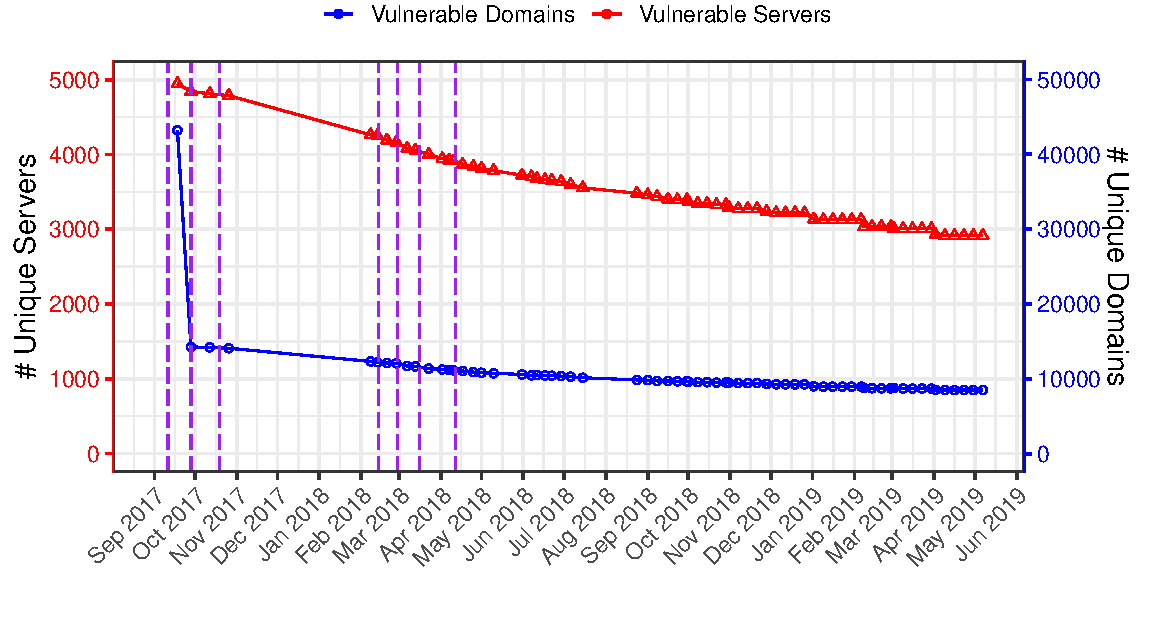
\includegraphics[width=\columnwidth]{figs/ts_notif.pdf}
    \caption{Number of vulnerable resources over time. Each dashed line represents a notification campaign.}
    \label{fig:ts_notif}
\end{figure}

\subsection{Notification methodology}



\subsection{Phase1: TF-CSIRTs}

\begin{table}[!htbp]
    \centering
    \caption{Summary statistics by the end of the Phase 1}
    \label{tab:my_label}
    \resizebox{\columnwidth}{!}{%
\begin{tabular}{lrr}
\toprule
 & TF-CSIRTs (N = 44) & Other CSIRTs (N = 36)\\
\midrule
\bf{Remediated Servers} & ~ & ~\\
\hline
~~ N (\%) & 328 (20.4)\% & 658 (19.17)\%\\
~~ max & 62 & 220\\
~~ median & 3.0 & 2.5\\
~~ mean (sd) & 7.45 $\pm$ 11.71 & 18.28 $\pm$ 39.10\\
\hline
\bf{Vulnerable Servers} & ~ & ~\\
\hline
~~ N (\%) & 1280 (79.6)\% & 2775 (80.83)\%\\
~~ max & 235 & 911\\
~~ median & 14.5 & 13.0\\
~~ mean (sd) & 29.09 $\pm$ 43.03 & 77.08 $\pm$ 172.45\\
\hline
\bf{Remediated Domains} & ~ & ~\\
\hline
~~ N (\%) & 737 (14.24)\% & 2173 (22.29)\%\\
~~ max & 108 & 847\\
~~ median & 4.0 & 4.5\\
~~ mean (sd) & 16.75 $\pm$ 27.41 & 60.36 $\pm$ 151.84\\
\hline
\bf{Vulnerable Domains} & ~ & ~\\
\hline
~~ N (\%) & 4439 (85.76\%) & 7574 (77.71\%)\\
~~ max & 1231 & 2384\\
~~ median & 29.5 & 34.0\\
~~ mean (sd) & 100.89 $\pm$ 195.19 & 210.39 $\pm$ 494.86\\
\bottomrule
\end{tabular}}
\end{table}


\begin{figure}[!hbt]
\centering
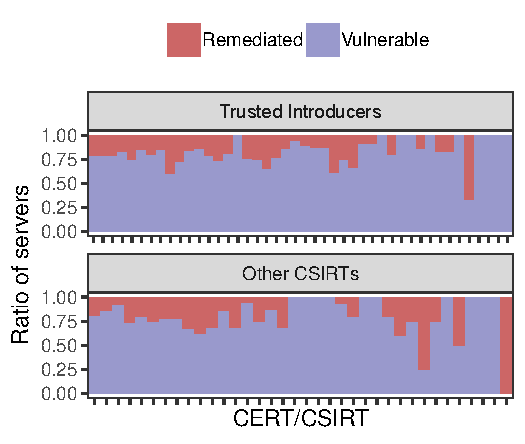
\includegraphics[width=.8\columnwidth]{distr_cleanup_1stcampaign.pdf}
\caption{Remediation rate of the DNS servers during the first campaign}
\end{figure}

\begin{figure}[!hbt]
\centering
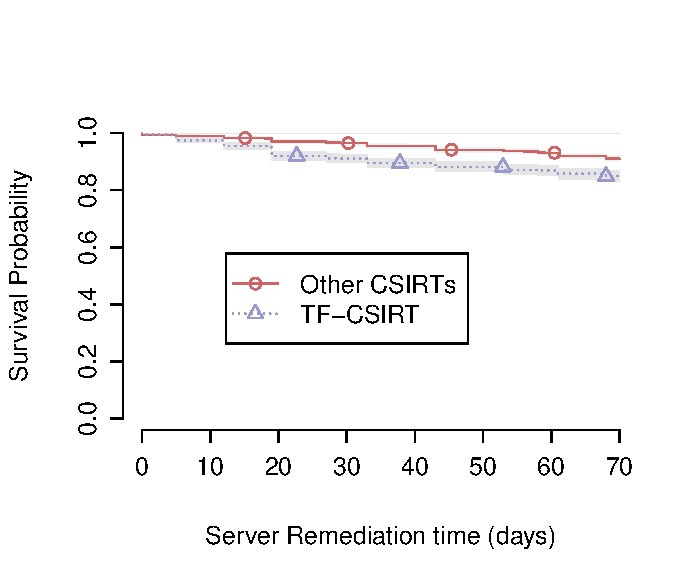
\includegraphics[width=.8\columnwidth]{tfcsirt_server.pdf}
\caption{Remediation rate of the DNS servers during the first campaign}
\end{figure}

\begin{figure}[!hbt]
\centering
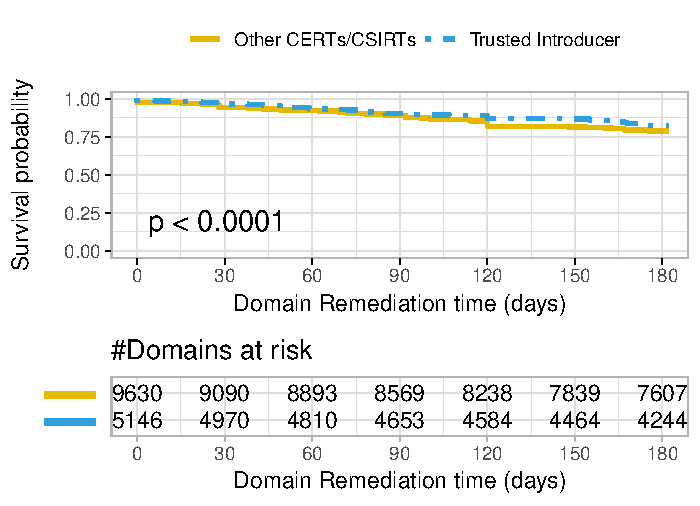
\includegraphics[width=.8\columnwidth]{tfcsirt_domain.pdf}
\caption{Remediation rate of the domains during the first campaign }
\end{figure}
\begin{figure}[!hbt]
\centering
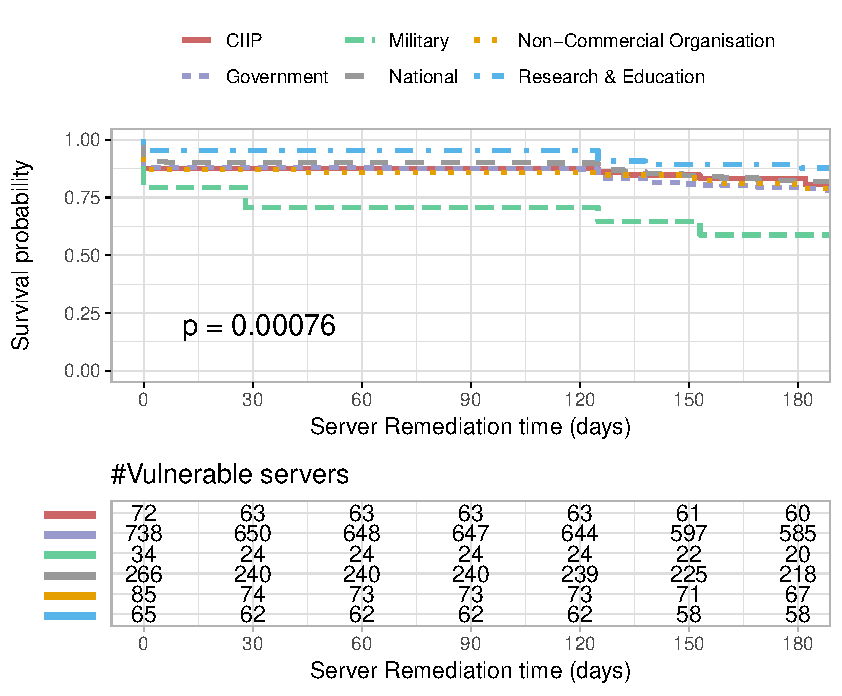
\includegraphics[width=.8\columnwidth]{figs/surv_tfcsirt-types.pdf}
\caption{Server remediation rate depending of the CSIRT constituency type }
\end{figure}


\subsection{Analyzing the remediation success}
\subsection{Lessons learned}
\section{Related work}


\subsection{DNSSEC}
\cite{goldberg2015nsec5} - The paper studes DNSSEC with NSEC and NSEC3 records, and shows that it inherently suffers from zone enumeration. They then propose a new construction that uses online public-key cryptography to solve the problem of DNSSEC zone enumeration - NSEC5
\cite{fiebig2017something} - We collect a new IPv6 addresses dataset spanning more than 5.8 million IPv6 addresses by exploiting DNS’ denial of existence semantics (NXDOMAIN).
\cite{kuhrer2015going} - research open DNS resolvers and found that many of them are malicious
\cite{moura2016anycast} - Evaluation of the DNS root event on Nov. 30 and Dec. 1, 2015.
\cite{schomp2014assessing} - Assessing DNS vulnerability to record injection with different attacks (but not dynamic updates)
\cite{pearce2017global} - Global measurement of dns manipulation
\cite{hao2018end} - DNS manipulation using dynaming mapping used by CDNs


\cite{van2015making} - studies DNSSEC reflection attack and blames RSA for that. They want to replace it by  elliptic curve cryptography (EC-DSA and EdDSA) are highly attractive for use in DNSSEC.
\cite{rasti2015temporal} - We introduce temporal lensing—a technique that concentrates a relatively low-bandwidth flood into a short, high-bandwidth pulse. Use this to perform DNS reflection attack. 
\cite{van2014dnssec} - Reflection attack using DNSSEC
\cite{macfarland2015characterizing} - Characterizing optimal DNS amplification attacks and effective mitigation
\cite{rossow2014amplification} - DNS reflections attack study using DNS DNSSEC and others. 




\cite{liang2013measuring} - measuring QoS of DNS root servers. 
\cite{osterweil2012behavior} - Behavior of DNS’Top Talkers, a .com/.net View
\cite{jonker2016measuring} - In this paper, we investigate the adoption of cloud-based DPSs worldwide. We focus on nine leading providers. Our outlook on adoption is made on the basis of active DNS measurements. We introduce a methodology that allows us, for a given domain name, to determine if traffic diversion to a DPS is in effect. It also allows us to distinguish various methods of traffic diversion and protection. 


Multiple studies focus on detection and clasification of  short-live domains automatically registrated by malwares \cite{vissers2017exploring,kountouras2016enabling,pereira2018dictionary,alrwais2014understanding,plohmann2016comprehensive,schuppen2018fanci}


\cite{zhang2014mismanagement} Utilizing Internet-scale measurements of DNS resolvers, BGP routers, and SMTP, HTTP, and DNS-name servers, we find there are thousands of networks where a large fraction of network services are misconfigured. 
\cite{dietrich2018investigating} - Measurements on network and DNS missconfiguration, why and how to protect.
\cite{borgolte2018cloud} - checking stale DNS records from old cloud services that were moved. Attackers can get those IP and get the traffic. 
\cite{lever2016domain} - analysing expired domains that are being registered by malicious attackers to highjack traffic. 
\cite{korczynski2016zone} - our previous paper
\cite{korczynski2017reputation} - Reputation metrics design to improve intermediary incentives for security of tlds



\cite{lever2013core} - try to find malware on mobile devices by analysing DNS. 
\cite{fukuda2015detecting} - Detecting Malicious Activity with DNS Backscatter (rDNS).





%%%%%%%%%%%%%%%%%% MEASUREMENTS %%%%%%%%%%%%%%%%%%%%%%%%%%%%%%%%%%%%%%%%
\subsection{Measurements}
\cite{schomp2013measuring} - measuring DNS client behaviour, caching etc. 
\cite{jones2016detecting} - We present techniques for detecting unauthorized DNS root servers in the Internet using primarily endpoint-based measurements from RIPE Atlas, supplemented with BGP routing announcements from RouteViews and RIPE RIS. 
\cite{fiebig2018rdns} - We observe that the share of non-authoritatively answerable IPv4 rDNS queries reduced since earlier studies and IPv6 rDNS has less non-authoritatively answerable queries than IPv4 rDNS. Furthermore, we compare passively collected datasets with actively collected ones, and we show that they enable observing the same effects in rDNS data. While highlighting oppor- tunities for future research, we find no immediate challenges to the use of rDNS as active and passive data-source for Internet measurement research.
%DNSSEC adoption/verification
\cite{lian2013measuring} - DNSSEC on client name resolution using an. A relatively small fraction of users are protected by DNSSEC-validating resolvers. and enabling DNSSEC measurably increases end-to-end resolution failures.
\cite{wander2013measuring} - checking whether a client is protected by DNSSEC validation. We applied our methodology over a period of 7 months collecting results from different data sources. 
\cite{chung2017understanding} - Looking at DNSSEC adoption
\cite{chung2017longitudinal} - A longitudinal, end-to-end view of the DNSSEC ecosystem
\cite{liu2018answering} - Understanding and characterizing interception of the DNS resolution path



\cite{zhu2015connection} - they propose to use TCP for DNS. That's a similar conclusion to ours. 








\section{Conclusions}

\bibliographystyle{IEEEtranS}
%TODO: add file for biblio
\bibliography{imcbib,biblio} 

\end{document}
